%% DESIGN: Inter (via Fira Sans fallback) | Young/fresh, projects-prominent | Bright blue (#2196F3) accent
\documentclass[11pt,a4paper]{article}
\usepackage[left=0.6in,right=0.6in,top=0.5in,bottom=0.5in]{geometry}
\usepackage[T1]{fontenc}
\usepackage[sfdefault]{FiraSans}
\usepackage{xcolor,titlesec,enumitem,hyperref,tikz,multicol}

\definecolor{accent}{HTML}{2196F3}
\definecolor{ACCENT}{HTML}{2196F3}
\definecolor{lightblue}{HTML}{E3F2FD}
\hypersetup{colorlinks=true,urlcolor=accent}
\pagestyle{empty}

\titleformat{\section}{\large\bfseries\color{accent}}{}{0em}{}[\vspace{-0.5em}\textcolor{accent}{\rule{\linewidth}{2pt}}]
\titlespacing{\section}{0pt}{0.9em}{0.4em}

\begin{document}

% Fresh, energetic header
\noindent

\begin{tikzpicture}
\fill[accent] (0,0) rectangle (\textwidth,2);
% Decorative dots
\foreach \x in {1,2,...,8} {\fill[white,opacity=0.1] (\x*1.8,1) circle (0.6);}
\node[anchor=west,text=white,font=\Huge\bfseries] at (0.3,1.2) {PRIYA SHARMA};
\node[anchor=west,text=white!90,font=\large] at (0.3,0.4) {Software Engineer | CS '2024};
\node[anchor=east,text=white!80,font=\small] at (\textwidth-0.3,1.2) {priya.sharma@email.com};
\node[anchor=east,text=white!80,font=\small] at (\textwidth-0.3,0.4) {github.com/priyasharma | (555) 012-3456};
\end{tikzpicture}

\vspace{0.5em}

\section{About}
Recent CS graduate passionate about building impactful software. Strong foundation in systems programming, web development, and machine learning. Active open-source contributor with 2 internship experiences at top tech companies.

\section{Education}
\noindent\textbf{B.S. Computer Science} \hfill \textcolor{accent}{University of Illinois at Urbana-Champaign, May 2024}\\
GPA: 3.85/4.0 \quad\textbar\quad Dean's List (all semesters) \quad\textbar\quad James Scholar Honors\\
\textbf{Relevant Coursework:} Distributed Systems, Machine Learning, Algorithms, Operating Systems, Databases, Computer Networks

\section{Projects}
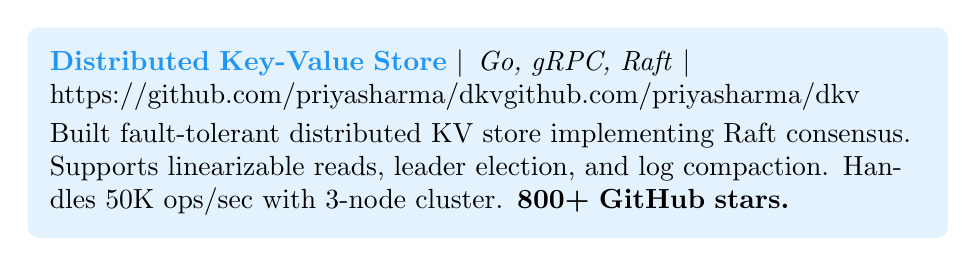
\begin{tikzpicture}
\node[fill=lightblue,rounded corners=4pt,inner sep=8pt,text width=\textwidth-1cm] {
\textbf{\color{accent}Distributed Key-Value Store} \textbar\, \textit{Go, gRPC, Raft} \textbar\, \href{https://github.com/priyasharma/dkv}{github.com/priyasharma/dkv}\\[2pt]
Built fault-tolerant distributed KV store implementing Raft consensus. Supports linearizable reads, leader election, and log compaction. Handles 50K ops/sec with 3-node cluster. \textbf{800+ GitHub stars.}
};
\end{tikzpicture}
\vspace{0.3em}

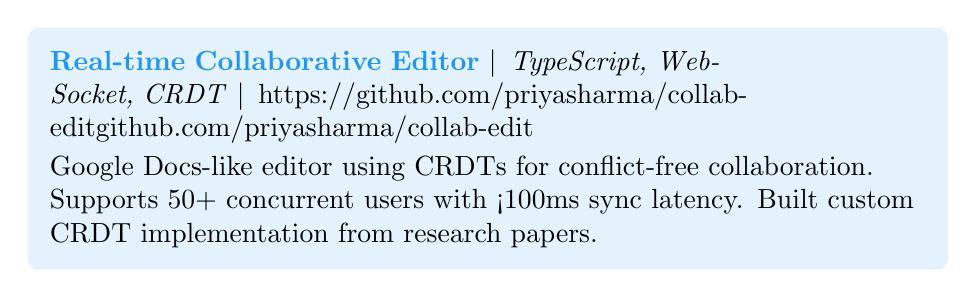
\begin{tikzpicture}
\node[fill=lightblue,rounded corners=4pt,inner sep=8pt,text width=\textwidth-1cm] {
\textbf{\color{accent}Real-time Collaborative Editor} \textbar\, \textit{TypeScript, WebSocket, CRDT} \textbar\, \href{https://github.com/priyasharma/collab-edit}{github.com/priyasharma/collab-edit}\\[2pt]
Google Docs-like editor using CRDTs for conflict-free collaboration. Supports 50+ concurrent users with <100ms sync latency. Built custom CRDT implementation from research papers.
};
\end{tikzpicture}
\vspace{0.3em}

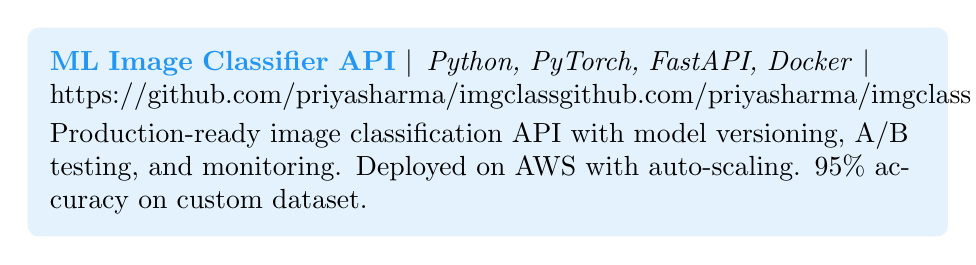
\begin{tikzpicture}
\node[fill=lightblue,rounded corners=4pt,inner sep=8pt,text width=\textwidth-1cm] {
\textbf{\color{accent}ML Image Classifier API} \textbar\, \textit{Python, PyTorch, FastAPI, Docker} \textbar\, \href{https://github.com/priyasharma/imgclass}{github.com/priyasharma/imgclass}\\[2pt]
Production-ready image classification API with model versioning, A/B testing, and monitoring. Deployed on AWS with auto-scaling. 95\% accuracy on custom dataset.
};
\end{tikzpicture}

\section{Experience}

\noindent\textbf{Software Engineering Intern} \hfill \textcolor{accent}{Summer 2023}\\
\textit{Google, Mountain View, CA}
\begin{itemize}[leftmargin=1.2em,nosep,label={\color{accent}\textbullet}]
\item Built feature for Google Maps reducing route calculation time by 15\% for complex queries
\item Implemented caching layer in C++ handling 1M+ requests/day; received return offer
\end{itemize}
\vspace{0.4em}

\noindent\textbf{Software Engineering Intern} \hfill \textcolor{accent}{Summer 2022}\\
\textit{Stripe, San Francisco, CA}
\begin{itemize}[leftmargin=1.2em,nosep,label={\color{accent}\textbullet}]
\item Developed internal tool for payment reconciliation, saving ops team 10 hours/week
\item Built with Ruby on Rails and React; deployed to production before internship end
\end{itemize}

\section{Skills}
\noindent\textbf{Languages:} Go, Python, C++, TypeScript, Java, Rust, SQL\\
\textbf{Technologies:} React, Node.js, Docker, Kubernetes, AWS, PostgreSQL, Redis, gRPC, GraphQL

\end{document}
